 \documentclass[12pt,a4paper]{article}

\usepackage{graphicx}% Include figure files
\usepackage{dcolumn}% Align table columns on decimal point
\usepackage{bm}% bold math
%\usepackage{hyperref}% add hypertext capabilities
%\usepackage[mathlines]{lineno}% Enable numbering of text and display math
%\linenumbers\relax % Commence numbering lines

%\usepackage[showframe,%Uncomment any one of the following lines to test 
%%scale=0.7, marginratio={1:1, 2:3}, ignoreall,% default settings
%%text={7in,10in},centering,
%%margin=1.5in,
%%total={6.5in,8.75in}, top=1.2in, left=0.9in, includefoot,
%%height=10in,a5paper,hmargin={3cm,0.8in},
%]{geometry}

\usepackage{multicol}%Para hacer varias columnas
\usepackage{multicol,caption}
\usepackage{multirow}
\usepackage{cancel}
\usepackage{hyperref}
\hypersetup{
    colorlinks=true,
    linkcolor=blue,
    filecolor=magenta,      
    urlcolor=cyan,
}

\setlength{\topmargin}{-1.0in}
\setlength{\oddsidemargin}{-0.3pc}
\setlength{\evensidemargin}{-0.3pc}
\setlength{\textwidth}{6.75in}
\setlength{\textheight}{9.5in}
\setlength{\parskip}{0.5pc}

\usepackage[utf8]{inputenc}
\usepackage{expl3,xparse,xcoffins,titling,kantlipsum}
\usepackage{graphicx}
\usepackage{xcolor} 
\usepackage{siunitx}
\usepackage{nopageno}
\usepackage{lettrine}
\usepackage{caption}
\renewcommand{\figurename}{Figura}
\usepackage{float}
\renewcommand\refname{Bibliograf\'ia}
\usepackage{amssymb}
\usepackage{amsmath}
\usepackage[rightcaption]{sidecap}
\usepackage[spanish]{babel}

\providecommand{\abs}[1]{\lvert#1\rvert}
\providecommand{\norm}[1]{\lVert#1\rVert}
\newcommand{\dbar}{\mathchar'26\mkern-12mu d}

\usepackage{mathtools}
\DeclarePairedDelimiter\bra{\langle}{\rvert}
\DeclarePairedDelimiter\ket{\lvert}{\rangle}
\DeclarePairedDelimiterX\braket[2]{\langle}{\rangle}{#1 \delimsize\vert #2}

% CABECERA Y PIE DE PÁGINA %%%%%
\usepackage{fancyhdr}
\pagestyle{fancy}
\fancyhf{}

\begin{document}

Macías Márquez Misael Iván

\begin{enumerate}



%%%1%%%



\item Considere un sistema formado por tres partículas iguales de masa $m$ que están localizadas en $(a,0,0)$, $(0,a,2a)$ y $(0,2a,a)$.a) Encuentre el tensor de inercia  (cheque que es una matriz de $3 \times  3$ simétrica).  b) Determine lo ejes principales de inercia y los correspondientes momentos principales de inercia.

\textbf{Sol:}

Recordando que el tensor  de inercia es

\begin{equation*}
    I _{\mu \nu} = \sum_{i = 1}^{3} m (r_{i}^{2} \delta_{\mu \nu} - x_{i \mu} x_{i  \nu})
\end{equation*}

entonces

\begin{equation*}
    I_{xx} = 10 m a^2
\end{equation*}

\begin{equation*}
    I_{yy} = I_{zz} = 6 m a^2
\end{equation*}



\begin{equation*}
    I_{xy} = I_{yx} = I_{xz} = I_{zx} = 0
\end{equation*}

\begin{equation*}
    I_{yz} = I_{zy} = -4ma^2 
\end{equation*}

o bien

\begin{equation*}
    I = \left( \begin{array}{lcc}
            10m a^2 & 0 & 0 \\
            \\ 0 & 6ma^2 & -4ma^2 \\
            \\ 0 & -4ma^2 & 6 ma^2 \\
        \end{array}
        \right)
\end{equation*}

donde

\begin{equation*}
    I^T = \left( \begin{array}{lcc}
            10m a^2 & 0 & 0 \\
            \\ 0 & 6ma^2 & -4ma^2 \\
            \\ 0 & -4ma^2 & 6 ma^2 \\
        \end{array}
        \right) = I
\end{equation*}

por lo que es simétrica, ahora encontremos los ejes principales y momentos principales de inercia

\begin{equation*}
    det(I - \lambda 1) = \left| \begin{array}{lcc}
            10m a^2 - \lambda & 0 & 0 \\
            \\ 0 & 6ma^2 - \lambda & -4ma^2 \\
            \\ 0 & -4ma^2 & 6 ma^2 - \lambda \\
        \end{array}
        \right| = (10ma^2 - \lambda) [(6ma^2 - \lambda)^2 - (4ma^2)^2]
\end{equation*}

\begin{equation*}
    = (10ma^2 - \lambda)^2 (4ma^2 - \lambda)^2 = 0
\end{equation*}

por lo que sus momentos principales de inercia son $\lambda_1 = \lambda_2 =10ma^2$ y $\lambda_3 = 4ma^2$ y ejes principales

\begin{equation*}
    \left( \begin{array}{lcc}
            10m a^2 \\
            \\ 0 \\
            \\ 0\\
        \end{array}
        \right)  , \left( \begin{array}{lcc}
            0 \\
            \\ 10 m a^2 \\
            \\ 0\\
        \end{array}
        \right),
        \left( \begin{array}{lcc}
            0\\
            \\ 0 \\
            \\ 4ma^2\\
        \end{array}
        \right) 
\end{equation*}







%%%2%%%



\item Determine la frecuencia  de las oscilaciones pequeñas de un cuerpo rígido que oscila alrededor de un eje horizontal fijo, bajo el efecto de la gravedad. El centro de masa está a una distancia $l$ del eje de rotación.

\textbf{Sol:}

Supongamos que la masa total es $M$ y el momento de inercia del eje de rotación $I_x = I$, entonces para este problema las ecuaciones de Euler quedan como 

\begin{equation*}
    I_{x'} \dot{\omega}_{x'} - \omega_{y'} \omega_{z'} (I_y - I_z) = N_x
\end{equation*}

y como el cuerpo rígido esta limitado a oscilar sobre un plano, podemos decir que $\omega_{y'} = \omega_{z'} = 0$ por lo que tenemos

\begin{equation*}
    I \ddot{\theta} = - Mgl \sin{\theta}
\end{equation*}

con$\theta$ el ángulo formado por el eje del cuerpo rígido y la vertical, ahora para pequeñas oscilaciones $\sin{\theta} \approx \theta$ y así

\begin{equation*}
    \ddot{\theta} + \frac{Mgl}{I} \theta = 0
 \end{equation*}
 
 y por lo tanto la frecuencia es
 
 \begin{equation*}
     \omega = \sqrt{\frac{Mgl}{I}}
 \end{equation*}



%%%3%%%





\item 

\begin{enumerate}
    \item Obtenga la energía cinética de un cilindro homogéneo de radio $a$ que rueda sin deslizar en el interior de una superficie cilíndrica de radio $R$ 
    
    \textbf{Sol:}
    
    \item Halle la frecuencia de las oscilaciones pequeñas $(\phi << 1)$ alrededor del punto de equilibrio
    
    \textbf{Sol:}
    
    \begin{figure}[h!]
    \centering
    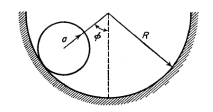
\includegraphics{3.PNG}
\end{figure}
    
\end{enumerate}



%%%4%%%



\item Un cilindro de radio $R$ que rueda sobre una mesa tiene una masa $M$ distribuida de modo tal que uno de los ejes principales de inercia es paralelo al eje del cilindro y está a una distancia $a$ de este. El momento de inercia relativo a dicho eje es $I$.

\begin{figure}[h!]
    \centering
    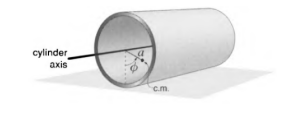
\includegraphics{4.PNG}
\end{figure}

\begin{enumerate}
    \item Encuentre la energía cinética total $T(\phi,\dot{\phi})$
    
    \textbf{Sol:}
    
    \item Determine el lagrangiano y la frecuencia de las oscilaciones pequeñas alrededor del punto de equilibrio.
    
    \textbf{Sol:}
    
    \item Si $a \rightarrow 0$ el centro de masa se localizará en el eje del cilindro. En este caso ¿qué espera que ocurra con la frecuencia de las oscilaciones pequeñas? ¿La expresión general obtenida en el inciso (c) reproduce este caso límite?
    
    \textbf{Sol:}
\end{enumerate}



%%%5%%%



\item Usando las ecuaciones de Euler, determine el torque necesario para rotar un cuerpo rectangular uniforme de masa $m$ con respecto a una diagonal con la velocidad angular constante $\omega$. Ignore el espesor del cuerpo y la gravedad.

\begin{figure}[h!]
    \centering
    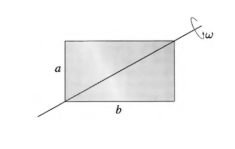
\includegraphics{5.PNG}
\end{figure}

\textbf{Sol:}



%%%6%%%



\item Una partícula de masa $m$ se mueve bajo el efecto de la gravedad $g$ a lo largo de la espiral $z = k \theta$, $r = R$, donde $k$ y $R$ son constantes, y $z$ es la dirección vertical.

\begin{enumerate}
    \item Encuentre el hamiltoniano $H(z,p)$ de la partícula.
    
    \textbf{Sol:}
    
    \item Determine y resuelva las ecuaciones de Hamilton.
    
    \textbf{Sol:}
    
    \item Muestre que en el límite $r \rightarrow 0$, $\ddot{z} = -g$
    
    \textbf{Sol:}
    
\end{enumerate}



%%%7%%%



\item Dos partículas de diferentes masa $m_1$ y $m_2$ están conectadas por un resorte de masa despreciable, constante elástica $k$ y longitud de equilibrio $d$. Este sistema se mueve sobre una mesa sin fricción y puede oscilar y rotar.

\begin{enumerate}
    \item Halle las ecuaciones de Lagrange
    
    \textbf{Sol:}
    
    \item ¿Existen coordenadas ignorables? ¿Cuáles son las cantidades de movimiento conjugadas?
    
    \textbf{Sol:}
    
    \item Determine el hamiltoniano y las ecuaciones de Hamilton.
    
    \textbf{Sol:}
    
\end{enumerate}



%%%8%%%



\item Sea $\phi (\mathbf{r}, \mathbf{p})$ una función esféricamente simétrica respecto al origen (invariante bajo rotaciones).

\begin{enumerate}
    \item $\phi$ depende de las componentes de $\mathbf{r}$ y $\mathbf{p}$ solamente a través de las combinaciones $\mathbf{r}^2$, $\mathbf{p}^2$ y $\mathbf{r}\cdot \mathbf{p}$. ¿Por qué?
    
    \textbf{Sol:}
    
    \item Demuestre que $[\phi, L_z] = 0$ donde $L_z$ es la componente $z$ del momento angular.
    
    \textbf{Sol:}
\end{enumerate}



%%%9%%%



\item \begin{enumerate}
    \item Verifique que la transformación 
    
    \begin{equation*}
        x = \frac{1}{\sqrt{m\omega}} (\sqrt{2P_1}\sin{Q_1} + P_2) \hspace{1cm} y = \frac{1}{\sqrt{m\omega}} (\sqrt{2P_1} \cos{Q_1} + Q_2)
    \end{equation*}
    
    \begin{equation*}
        P_x = \frac{1}{2} \sqrt{m \omega} (\sqrt{2P_1} \cos{Q_1} - Q_2) \hspace{1cm} P_y = \frac{1}{2}\sqrt{m \omega} (- \sqrt{2P_1}\sin{Q_1} + P_2)
    \end{equation*}
    
    es canónica
    
    \textbf{Sol:}
    
    \item Halle las ecuaciones de Hamilton para una partícula de masa $m$ y carga $e$ que se mueve en el plano $xy$ en presencia de un campo magnético descrito por el potencial vector
    
    \begin{equation*}
        A(\mathbf{r}) = \left(- \frac{yB}{2} , \frac{xB}{2},0\right)
    \end{equation*}
    
    en términos de las nuevas variables $Q_1$, $Q_2$, $P_1$, $P_2$ y con $\omega = \frac{eB}{m}$
    
    \textbf{Sol:}
    
    
\end{enumerate}



%%%10%%%



\item Una partícula (con masa $m=1$) se mueve en un potencial unidimensional de la forma

\begin{equation*}
    V(x) = U \tan{ax}
\end{equation*}

donde $U$ y $a$ son constantes.

\begin{enumerate}
    \item Determine los puntos de retorno.
    
    \textbf{Sol:}
    
    \item Demuestre que la variable de acción $I$ obedece la relación
    
    \textbf{Sol:}
    
    \begin{equation*}
        \frac{aI}{\sqrt{2}} = \sqrt{E + U} - \sqrt{U}
    \end{equation*}
    
    donde $E$ es la energía total.
    
    \item Pruebe que la frecuencia $\omega$ depende de la energía como
    
    \begin{equation*}
        \frac{\omega}{a \sqrt{2}} = \sqrt{E+U}
    \end{equation*}
    
    Explique por qué la frecuencia aumenta con la energía.
    
    \textbf{Sol:}
    
\end{enumerate}
    
    
\end{enumerate}

\end{document}
